\documentclass[11pt]{preprint}

\setlength{\topmargin}{0mm} \setlength{\oddsidemargin}{0mm}
\setlength{\textwidth}{160mm} \setlength{\textheight}{215mm}

\usepackage{amssymb,amsmath,amscd,amsthm}
\usepackage{tikz}
\usepackage{wrapfig}

\newtheorem{proposition}{Proposition}
\newtheorem*{solution}{Solution}

\def\enumb{\begin{enumerate}}
\def\enume{\end{enumerate}}
\def\integers{\mathbb{Z}}
\def\multiset#1#2{\ensuremath{\left(\kern-.3em\left(\genfrac{}{}{0pt}{}{#1}{#2}\right)\kern-.3em\right)}}

\title{Discrete Mathematics, 2016 Fall - HW 13 (Optional)}
\author{Instructor: Zsolt Pajor-Gyulai}
\institute{Courant Institute of Mathematical Sciences, NYU}



\begin{document}

\maketitle

To get full credit  in all of the problems, use rigorous justification and unless otherwise indicated, make sure that your solution reads as a perfect English sentence. You should only assume integers, operations and order relations as given. If you use a statement or a definition from the textbook, make sure to indicate it.
\vspace{0.2cm}


\textbf{Section 49}
\enumb
\item[4)] Let $n\geq 2$ be an integer. Form a graph $G_n$ whose vertices are all the two-element subsets of $\{1,2,\dots,n\}$. In this graph, we have an edge between distinct vertices $\{a,b\}$ and $\{c,d\}$ exactly when $\{a,b\}\cap\{c,d\}=\emptyset$.
\enumb
\item How many vertices does $G_n$ have?
\begin{solution}
By definition, there are $\binom{n}{2}$ two element subsets and therefore
\[
|V(G_n)|=\binom{n}{2}
\]
\end{solution}
\item How many edges does $G_n$ have?
\begin{solution}
There are $\binom{n}{2}$ choices for one end of the edge and the other end can be chosen as any two element subset from the remaining $n-2$ elements. However this way we double count every edge (once as $ab$ then as $ba$) and thus
\[
|E(G_n)|=\frac{1}{2}\binom{n}{2}\binom{n-2}{2}
\]
\end{solution}
\item For which values of $n\geq 2$ is $G_n$ connected? Prove your answer.
\begin{solution}
You can check directly that $G_2$ and $G_3$ are edgeless graphs, while $G_4$ has three connected components. However, we claim that $G_n$ is connected for $n\geq 5$. Indeed, in this case take $\{a,b\}, \{c,d\}\in V(G_n)$ arbitrary. If $a,b,c,d$ are all different numbers then clearly $\{a,b\}$ and $\{c,d\}$ are adjacent and the edge between them is a path connecting them. If however $b=c$, then as $n\geq 5$, there exist $e,f$ different from $a, b=c, d$, and therefore
\[
\{a,b\}\sim\{e,f\}\sim\{c,d\}
\]
gives a path between $\{a,b\}$ and $\{c,d\}$. This shows that $G_n$ is connected.
\end{solution}
\enume
\item[6)] Let $G$ be a graph. A path $P$ in $G$ that contains all the vertices of $G$ is called a \textbf{Hamiltonian path}. Prove that the following graph does not have a Hamiltonian path. 
\begin{figure}[ht]
\centering
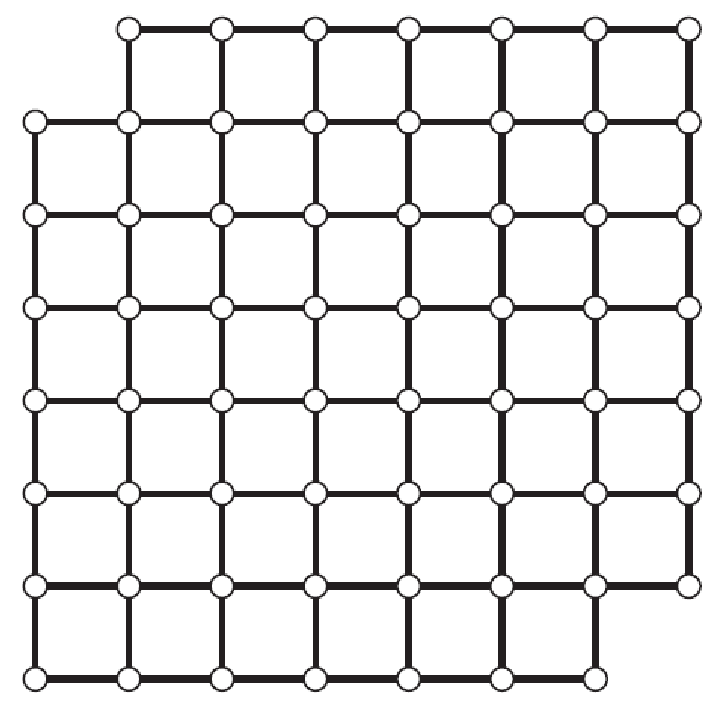
\includegraphics[scale=0.3]{HW1.pdf}
\end{figure}

\begin{solution}
Color the vertices in a checkerboard pattern. Then every walk in every step must move between black and white vertices and therefore the number of touched black and white vertices must be the same or differ by one. However, there are 32 black vertices and 30 whites and therefore no path can traverse all.
\end{solution}


\item[10)] Let $G$ be a graph. Prove that $G$ or $\bar{G}$ or both must be connected.

\begin{solution}
If $G$ is connected, there is nothing to prove so assume $G$ is not connected. Then it has at least two nonempty connected component and as a result, there are vertices $x$ and $y$ in different components of $G$ (meaning also that $x$ and $y$ are adjacent in $\bar{G}$. 

Take arbitrary $a,b\in V(\bar{G})=V(G)$. We show that there is a path connecting them in $\bar{G}$. There are three cases
\begin{itemize}
\item If $a$ and $b$ are both in $x$'s component then they are both adjacent to $y$ in $\bar{G}$ and
\[
a\sim y\sim b
\]
provides such a path.
\item If none of them are in $x$'s component then they are both adjacent to $x$ in $\bar{G}$ and
\[
a\sim x\sim b
\]
provides such a path.
\item If one of them, let's say $a$, is in $x$'s component and the other one is not, then $a$ is adjacent to $y$ and $b$ is adjacent to $x$ and therefore
\[
a\sim y\sim x\sim b
\]
provides such a path.
\end{itemize}
\end{solution}
\enume

\textbf{Section 50}
 \enumb 
\item[5)] Let $e$ be an edge of a graph $G$. Prove that $e$ is not a cut edge if and only if $e$ is in a cylce of $G$.
\begin{solution}~

\begin{enumerate}
\item[($\Leftarrow$):] If the edge $e=xy$ is in a cycle, then we can get from $x$ to $y$ by traversing $e$ directly or we can go around the other way along the cycle. The latter survives if we cut $e$ and therefore $e$ is not a cut edge.
\item[($\Rightarrow$):] If the edge $e=xy$ is not a cut edge then there is an $(x,y)$ path $P$ in $G-e$. But then $P^{-1}+e$ is a cycle that contains $e$.
\end{enumerate}
\end{solution}
\item[10)] Prove that a graph is a forest if and only if all of its edges are cut edges.
\begin{solution}
If a graph is a forest then there are no cycles and by the previous problem all edges are cut edges. On the other hand if all edges are cut edges then no edge in the graph can be in a cycle and therefore the graph is acyclic, i.e. a forest.
\end{solution}

\item[16)] Let $G$ be a graph. A cycle of $G$ that contains all the vertices in $G$ is called a \textbf{Hamiltonian cycle}.
\enumb
\item Show that $n\geq 5$, then $\bar{C}_n$ has a Hamiltonian cycle.
\begin{solution}
Come and I'll draw this two you.
\end{solution}

\item Prove that the graph in the figure does not have a Hamiltonian cycle.
\enume
\begin{figure}[ht]
\centering
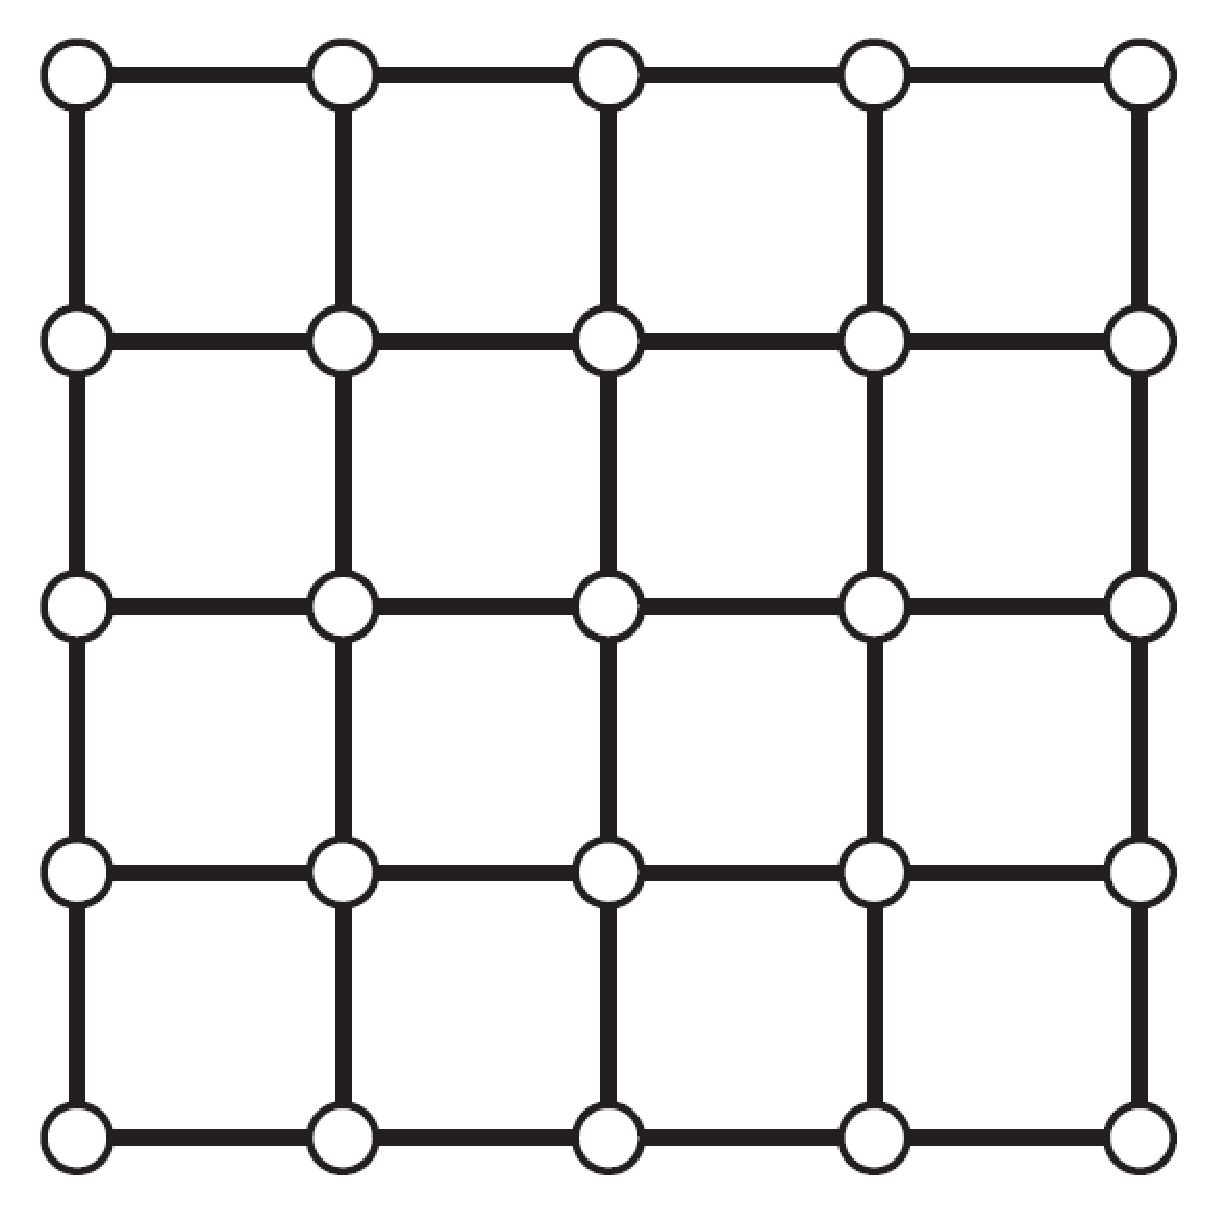
\includegraphics[scale=0.22]{HamltonCirc.pdf}
\end{figure}
\enume
\begin{solution}
Again color the vertices according to a checkerboard pattern. Since every walk must move between black and white vertices at each step, every cycle must have an even length. However, there are $25$ vertices here so a Hamiltonian cycle would have to have length $25$. $\Rightarrow\Leftarrow$.
\end{solution}
\textbf{Section 51}

\enumb
\item [6)] Let $G$ be an Eulerian graph. Prove that it is possible to partition the edge set of $G$ such that the edges in each part of the partition form a cycle of $G$.
\begin{solution}
Let $P$ be an Eulerian tour. Then segments of this tour between vertex repetitions are cycles. Since the tour is Eulerian, eventually we exhaust all the edges and therefore these cycles form a partition of the edge set.
\end{solution}
\item [7)] A rook is a chess piece that may, on a single turn, move any number of squares horizontally or any number of squares vertically on the board. That is, if squares $A$ and $B$ are in the same row [or same column] then we are permitted to move the rook from $A$ to $B$. Other moves, however, are illegal. Thus in every row and every column there are $\binom{8}{2}$ pairs of squares between which the rook may move. This gives a total of $16\binom{8}{2}=448$ such pairs.

Suppose a rook is placed on an empty chess board. Can we repeatedly move the rook so that it moves exactly once between each pair of squares in the same row and once between each pair of squares in the same column?

\begin{solution}
This is a problem that looks super complicated, however, can be answered in a simple way by rephrasing it as a graph theory problem. Let $G=(V,E)$ be a graph, where $V$ is the set of all fields in the chessboard, thus $|V|=64$. Let the edge set consist of all the pairs of fields that are either in the same row or in the same column. Then $|E|=16\binom{8}{2}=448$, and the question in the problem boils down to the question whether there is an Eulerian trail in this graph. However, for a fixed field, there are $7+7=14$ legit moves for the rook and therefore $d(v)=14$ for all vertices in this graph, implying that there is even an Eulerian tour. This means that we have proved the stronger question when your rook also has to end up at the same place it started!
\end{solution}
\enume
\textbf{Section 52}

\enumb
\item[1)] Let $H$ be the graph in the following figure.
\begin{figure}[ht]
\centering
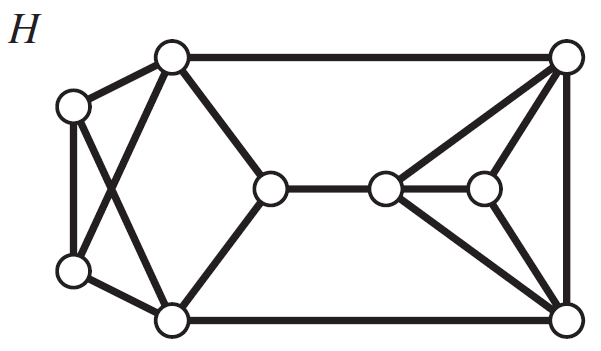
\includegraphics[scale=0.4]{Color1.jpg}
\end{figure}
Please find $\chi(H)$.
\begin{solution}
Clearly, you see $K_4$ on the right side of this graph, and therefore $\chi(H)\geq 4$. However, one can easily exhibit a four coloring (come and I'll show it to you) showing $\chi(H)\leq 4$ and the two together means $\chi(H)=4$.
\end{solution}
\item[8)] Let $G$ be a graph with $n$ vertices. Prove that $\chi(G)\geq\omega(G)$ and $\chi(G)\geq n/\alpha(G)$.

\begin{solution}
Since there is a clique of size $\omega(G)$, the complete graph $K_{\omega(G)}$ is a subgraph of $G$ which proves the first inequality. 

To show the second one, note that the vertices of the graph $V(G)$ can be partitioned into $\chi(G)$ different color classes. By the definition of proper coloring, vertices of the same color form an independent set. Therefore if $n_i$ is the number of vertices in the $i$th color class then $n_i\leq \alpha(G)$
\[
n=\sum_{i=1}^{\chi(G)}n_i\leq\chi(G)\max_{i=1,\dots,\chi(G)}n_i\leq \chi(G)\alpha(G)
\]
proving the second inequality. (Compare this with the proof that $n\leq\chi(G)\chi(\bar{G}))$.
\end{solution}

\item[14)] Suppose $G$ has maximum degree $\Delta>1$, but it has only one vertex of degree $\Delta$. Prove that $\chi(G)\leq\Delta$.
\begin{solution}
Color that one vertex first. Then color the remaining vertices one by one using $\Delta$ colors. You will never reach a conflict in this procedure since every remaining vertex has at most $\Delta-1$ neighbors and therefore it will always be possible to find a color on the palette of size $\Delta$ that is different from all the neighbor's colors.
\end{solution}
\enume

\end{document}